\section{Workflow}
As shown in Figure \ref{fig:teaser} left, our workflow starts from physically collecting branches.
In this section, we introduce two steps in the workflow shown in \ref{fig:teaser} left: Collecting and Scanning Branches (1 amd 2 in Figure~\ref{fig:teaser} left) and Fabrication (4 in Figure~\ref{fig:teaser} left).
As for the game (3 in Figure~\ref{fig:teaser} left), please refer Section \ref{sec:game}.
The collected branches are uploaded to cloud database by \textit{Branch Importer}, and served to the online game-based design application \textit{BranchConnect}.
The game system uses skeletons for its joint detection process, which works on browsers on laptop computers or mobile touch devices.
As shown in Figure \ref{fig:teaser} right, users can explore a global design with various layouts designed by multiple users.
Once layouts are selected the global design is fixed, these layouts are further inspected by \textit{G-Code Generator}, which generates customized joints for CNC milling.
After finishing the milling process, users physically assemble branches and complete the fabrication process.
The pipeline of the workflow is illustrated in the Figure \ref{fig:pipeline}.

\begin{figure}[ht]
  \begin{center}
    \includegraphics[width = 0.4\paperwidth]{images/workflow/pipeline.png}
    \caption{A pipeline from model acquisition to fabrication.}
    \label{fig:pipeline}
  \end{center}
\end{figure}

\subsection{Collecting and Scanning Branches}
Users can collect branches and upload to the online database.
Considering the mechanical constraints of CNC milling machine, branches are cut in certain length.
Please refer Section~\ref{sec:casestudy} for details.
The cut branches need to be firmly fixed to plates for milling process.
We use metal fixtures to attach them on a plate (See Figure~\ref{fig:skeleton}).
After attaching branches on plates, users can start scanning and acquire textured mesh model.
We describe the scanning setup further in details in Section~\ref{sec:casestudy}.

%As complete mesh model provides more robust results with 3D shapes of branches, we describe our process based on mesh model as an input.
Taking mesh model with colored texture, our \textit{Branch Importer} provides functions such as object detection, skeleton extraction, branch type classification, and fixture point setting.
The scanned result is a mesh model representing branches with a base plate.
The system first identifies branches by applying simple height threshold, and then applies contour detection.
The obtained 2D contours are used for extracting skeletons and clustering vertices in the mesh model.
Contours are triangulated and skeleton points are extracted from middle points on edges of triangles.
These middle points are compared with top view image.
If the point is inside of a contour, the middle point is counted as a skeleton point.
After extracting skeleton points, the connectivity of skeletons is analyzed.
In case grafting branch (Y-shaped branch) is detected, a new skeleton sub-branch is added.
The result is shown in Figure ~\ref{fig:skeleton}.
%Evaluating the number of sub-branches, the branch is morphologically classified.
Metal fixture locations are confirmed by simple mouse-clicks and marked as invalid, meaning that joints should not be placed on these points.
The acquired information is stored in a cloud database.

\begin{figure}[ht]
  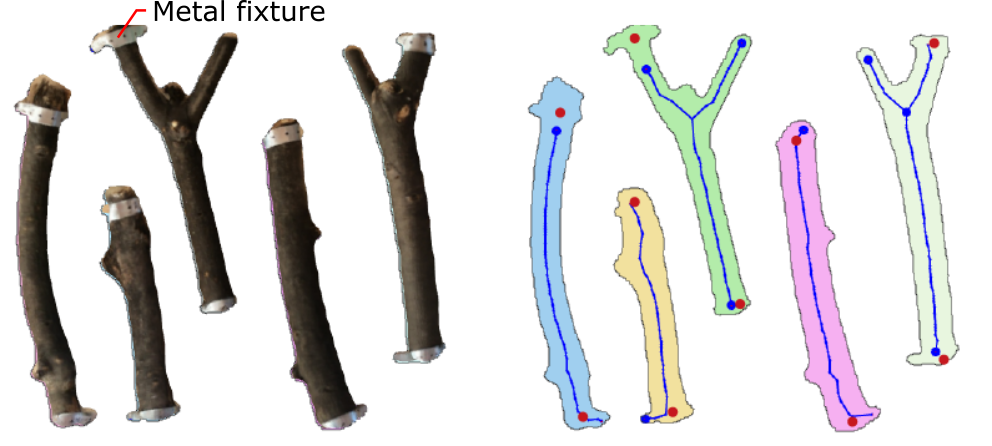
\includegraphics[width = 0.4\paperwidth]{images/importer/importer_2.png}
  \caption{An interface of \textit{Branch Importer}. Left: a top ortho-view image of textured mesh model. Right: Extracted skeletons are shown with blue dots. The beginning of skeletons is shown bigger dots, and the red dots are invalid points defined by a user. }
  \label{fig:skeleton}
\end{figure}


\subsection{Fabrication}
\label{sec:fabrication}
After a design is selected for fabrication, fabricatability of the design is further inspected by a high-resolution model.
The \textit{G-Code Generator} displays joints and milling paths on scanned orientations.
If it identifies an invalid joint in the high resolution model, a layout can be easily modified with simple mouse inputs (Figure \ref{fig:joint_geometry}.1 and \ref{fig:joint_geometry}.2).
Users can also change milling parameters such as offset ratio of milling paths, milling bit diameter, depth of joints, cutting speed, moving height and so forth.
After confirming the fabrication settings and milling paths, it generates G-Code.\\

Some fabrication factors such as invalid points due to metal fixtures and flipped (further described in Section \ref{sec:joint}) are already considered by \textit{Branch Importer} and the game system respectively.
Here, we describe the process to calculate joint geometry for fabrication.
The \textit{G-Code Generator} searches a set of four closest points on high-resolution contours (Figure \ref{fig:joint_geometry}.1).
By trimming contours of each branch at the corner points, we get \textit{side cuts} and \textit{center cuts} (Figure \ref{fig:joint_geometry}.4).
Please refer Appendix~\ref{sec:sidecut} for details of this process.
\textit{Side cuts} have wedged corners for smooth assembly process.
The depth of the \textit{center cuts} is half of the top height at the joint position from a mesh model (Figure \ref{fig:joint_geometry}.4).
The bottom height is usually the height of the base plate, however, in case of under-cuts with incomplete mesh model, we calculate a half of the diameter from the 2D contour and subtract it from the top height.
The resulting geometry creates rigid joints with irregularly shaped sections.


%\begin{figure}[ht]
%  \begin{center}
%    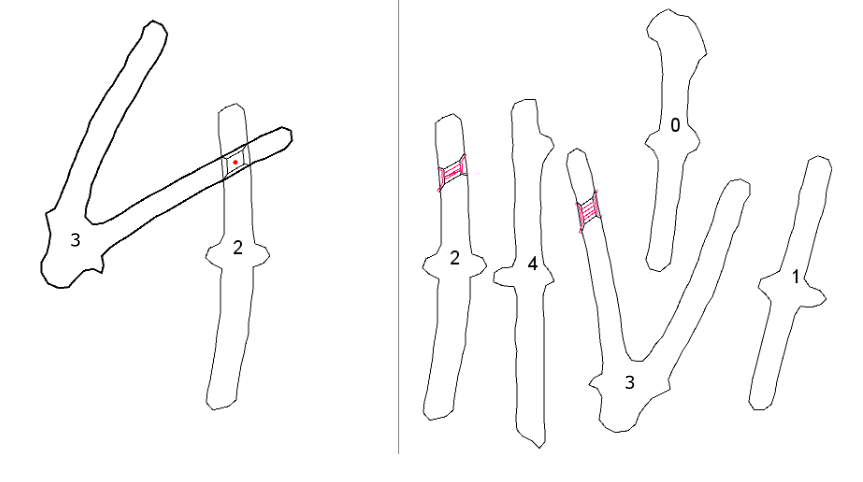
\includegraphics[width = 0.35\paperwidth]{images/system/gcode_generator_4.png}
%    \caption{The interface of \textit{G-Code Generator}. Left: a layout defined by a user. Right: the original orientations of branches with generated milling paths with red color. }
%    \label{fig:gcode_gen}
%  \end{center}
%\end{figure}

\begin{figure}[h]
	\begin{center}
		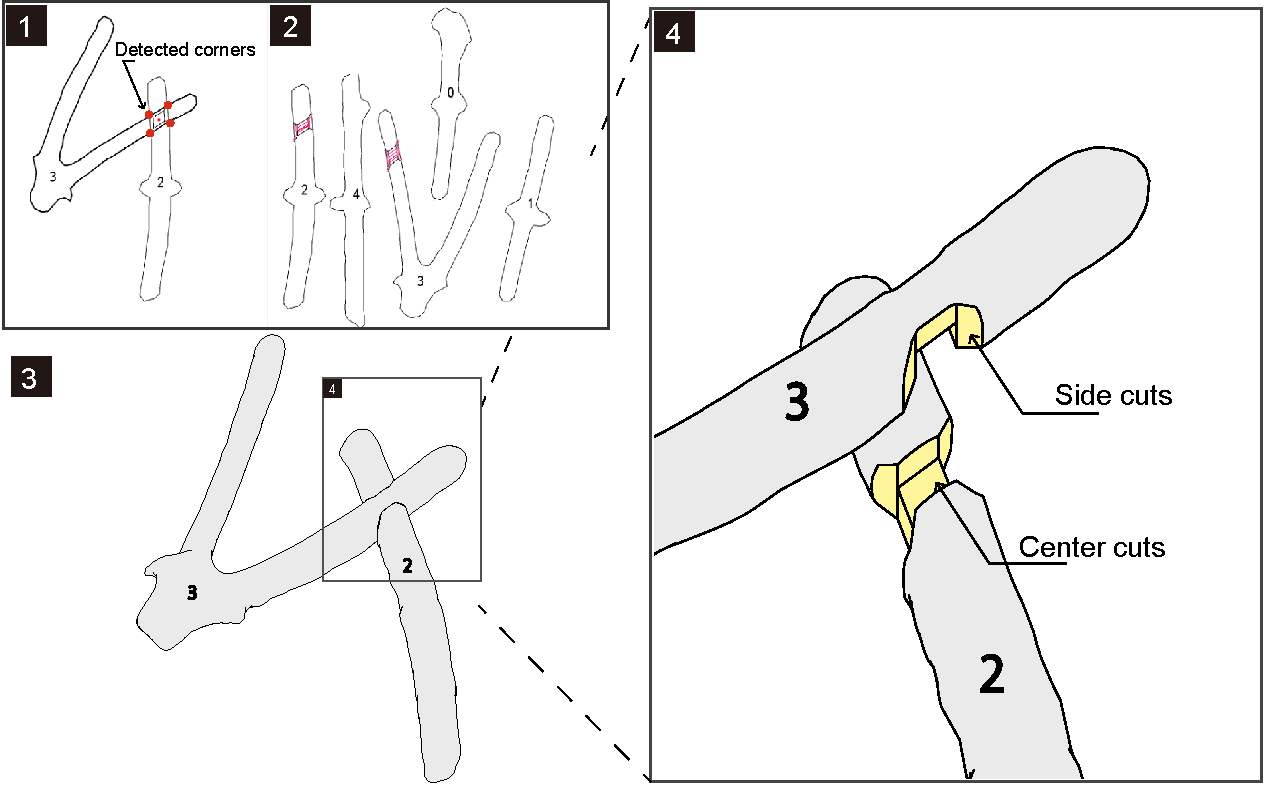
\includegraphics[width = 0.4\paperwidth]{images/system/joint_diagram.pdf}
		\caption{1, 2: an interface of G-Code Generator. 1. a layout defined by a user. 2. the original orientations of branches with generated milling paths with red color. 3. an assembled pair of branches with branch 3 is flipped. 4. milled branches with center cuts and side cuts.}
		\label{fig:joint_geometry}
	\end{center}
\end{figure}
